\documentclass[a4paper,11pt]{article}

\usepackage{graphicx}
\usepackage{natbib}

\title{Extended Bayesian Skyline Plot tutorial\\for BEAST 2}

\author{Joseph Heled\\(updated for BEAST 2 by Tim Vaughan)}
\date{}

\setlength{\parindent}{0em}
\setlength{\parskip}{1em}

\begin{document}

\maketitle

This short practical explains how to set up an Extended Bayesian Skyline Plot
(EBSP) analysis in BEAST 2 \citep{Bouckaert2014}, and how to generate some EBSP
plots.

To make the most of this tutorial you should follow the steps described here on
your system. Reading the article \citep{Heled2008} first is not a bad idea
either. Use your own data if you are comfortable with BEAST, otherwise use the
provided examples.  The next section uses the data in the `mystery-mammal'
directory, three genes from a small mammal: one nuclear, one mitochondrial, and
one from the X chromosome.

This tutorial is based on BEAST version 2.3.2. Before proceeding any further,
visit \texttt{www.beast2.org} and ensure you are running the latest version.

My sincere apologies for any harm done by the figures to your aesthetic
sensibilities. Nobody, the Java team included, cares much for my preferred
platform, Linux.

\section{Setting up the analysis}

\subsection{Loading the data}

The EBSP is a multi-locus method, so the step first involves loading all
loci/genes into BEAUti. The simplest way to do so is to prepare one NEXUS file
for each alignment. Taxa names in each alignment have to be unique, but
duplicates across alignments are fine.

Start BEAUti, open the File menu and select `Import Alignment`.  Navigate to
the data directory, select all the files you wish included in the analysis and
click `Open' (Figure~\ref{fig:importAlignment}).

\begin{figure}[h!]
    \centering
    \hspace{-0.5cm}\begin{minipage}[b]{0.4\textwidth}
        \begin{center}
            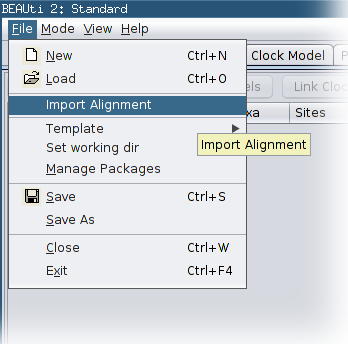
\includegraphics[width=\textwidth]{figures/import_alignment.png}
            (a)
        \end{center}
    \end{minipage}\hspace{0.5cm}\begin{minipage}[b]{0.6\textwidth}
        \begin{center}
            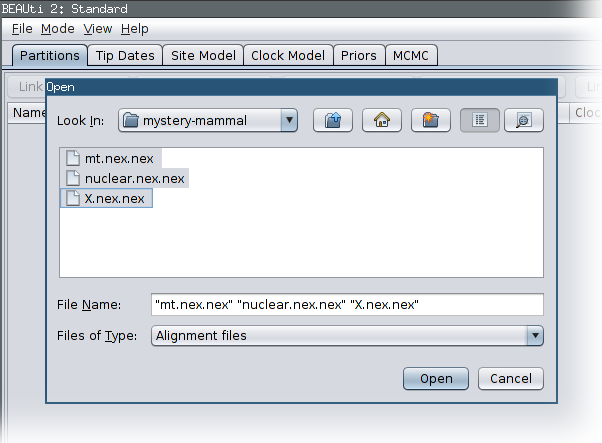
\includegraphics[width=\textwidth]{figures/import_alignment2.png}
            (b)
        \end{center}
    \end{minipage}
    \caption{Loading multiple alignments into BEAUti.}
\label{fig:importAlignment}
\end{figure}

\subsection{Site model}

Open the \textsc{Site Model} pane. Here we choose, for every gene, the
evolutionary models specifying how characters evolve at each site (one aligned
position). Do not automatically choose the most general models possible (GTR,
Gamma + Invariant Sites, Partitioned Codon positions etc.). Please remember
that the more general models have more parameters, and this may result in
longer runs and slower mixing. This is the time to display your superior
knowledge of the data! Sometimes performing an exploratory run(s) on a single
loci can help, especially when the simpler model is a special case of a general
one. Sometimes the simpler model is represented by particular parameter values,
and checking if the credible interval(s) contain those specific values can be a
factor in the decision.

In this particular case we'll use the HKY substitution model, but will change
the `Frequencies' to Empirical, as shown in the following figure:

    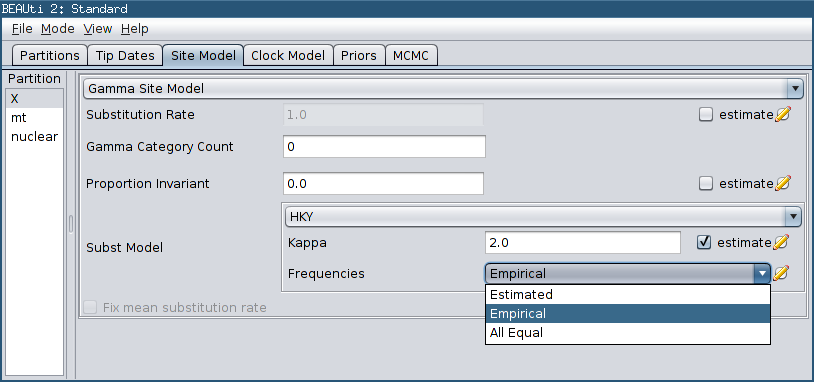
\includegraphics[width=\textwidth]{figures/site_model.png}

Repeat for each loci. Please note that I know absolutely nothing about
this particular data, and it is entirely possible using the GTR or partitioning
is the better choice.

\subsection{Clock model}

Now move to the \textsc{Clock Model} pane. Here you choose the molecular clock
model for each gene. The same considerations as in the site model apply: stay
with the strict clock unless you know otherwise.

You may have noticed that exactly two of the three genes are marked as
`Estimate'. In general we can't infer the absolute rate from contemporaneous
data (all samples collected at the same time), but we can infer relative rates.
The unmarked loci is the reference rate, which is by default set to one. Other
rates will be relative to the reference: a rate of 2 (with the reference being
1) means `evolving twice as fast as the reference'.

In general it is best to pick the most stable reference. Here this would be the
mtDNA, since it evolves faster, and so the sequences in that loci will be more
divergent and contain more information. Ensure that the rate of `mt.nex' is
unchecked and the other two are checked. To do this, you'll first need to open
the `Mode' menu and deselect `Automatic set clock rate', as shown below:

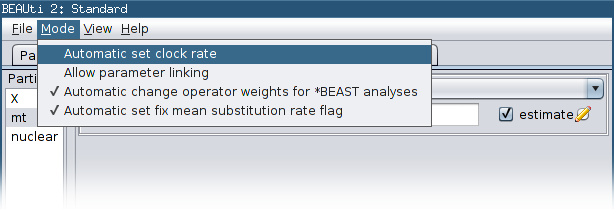
\includegraphics[width=\textwidth]{figures/clock_model.png}

Then, select each of the loci names in turn from the list on the left hand side
of the screen, making sure that `estimate' is checked for X and nuclear but
unchecked for mt, as shown in figures below:

\begin{center}
    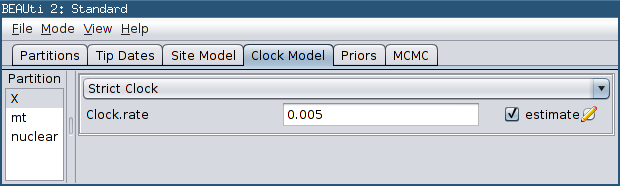
\includegraphics[width=0.8\textwidth]{figures/clock_model2.png}
\end{center}

\begin{center}
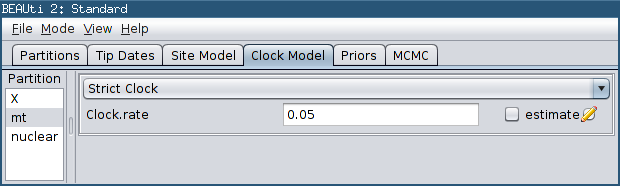
\includegraphics[width=0.8\textwidth]{figures/clock_model3.png}
\end{center}

\begin{center}
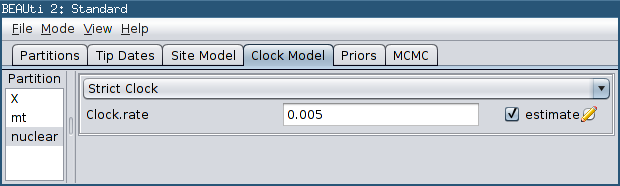
\includegraphics[width=0.8\textwidth]{figures/clock_model4.png}
\end{center}

The units of the time axis for the trees and population size is the same as the
reference rate. When it equals 1, time is measured in substitutions. When we
have an estimate of the reference, it may be more convenient to plug it in and
have time in years. Since this is a mammal, I will arbitrarily pick a rate of
0.05 per million years. Double-Click on the 1.0 rate for the mt locus and enter
0.05 – and times from the analysis will be in millions of years.

To make a smoother start you should change the other starting rates – say to
0.005.  Note that we set the reference rate to a known fixed value, but that
can be relaxed too. It is possible to let the rate vary (by checking it's
`Estimate' box as well), and place a prior on the rate parameter in the priors
section (which is clockRate.c:mt in this specific case). You have to realize
that the rate will not be estimated---there is no data here to make that
possible---it will simply follow the prior. But the uncertainty regarding the
exact value will be reflected in all other estimates.

\subsection{Priors}

Now, switch to the \textsc{Priors} pane. The first thing we need to do here is
set the prior for each of the gene trees to `Coalescent Extended Bayesian
Skyline`.  Do this by selecting this option from the drop-down menu to the
right of `Tree.t:X', `Tree.t:mt' and `Tree.t:nuclear', as shown below:

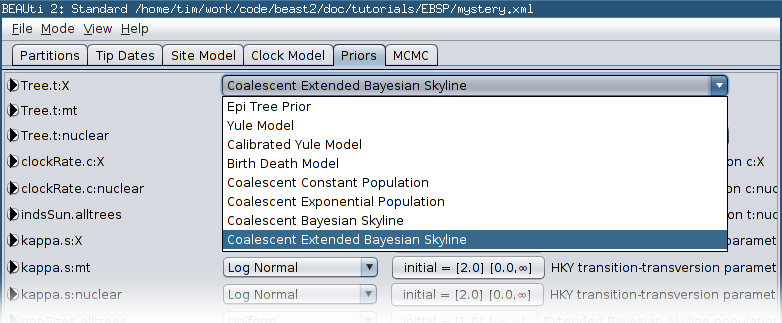
\includegraphics[width=\textwidth]{figures/tree_prior.png}

Once this is complete, click the arrow to the left of Tree.t:X, then click the
pencil icon to the right of the `PopulationModel' text that appears. As shown
in the following figure, this will bring up a dialog containing a text
field that allows you to edit the scale factor for the population size applied
to this particular gene tree:

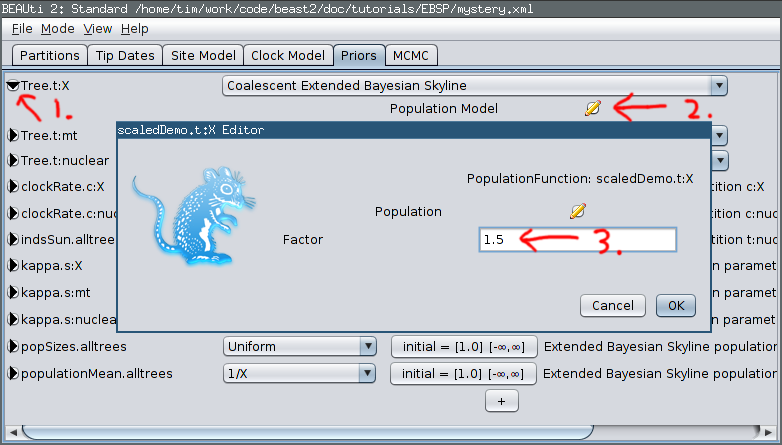
\includegraphics[width=\textwidth]{figures/ploidy.png}

This allows us to account for the ploidy of each locus. Since this gene is on
the X chromosome, we apply a scale factor of 1.5 as each member of the
population has 1.5 copies of this gene on average.

Perform these same steps to set the scale factors for the mtDNA and nuclear
genes to 0.5 and 2 respectively. (We use 0.5 for mtDNA because only the female
mtDNA contributes to the effective population size.)

Next, we replace the improper uniform priors on the two estimated clock rates
with proper uniform priors by setting a finite upper bound of 1.0 for each.  Do
this by clicking the arrows to the left of clockRate.c:X and
clockRate.c:nuclear and replacing `infinity' with 1.0, as shown in
the following figure:

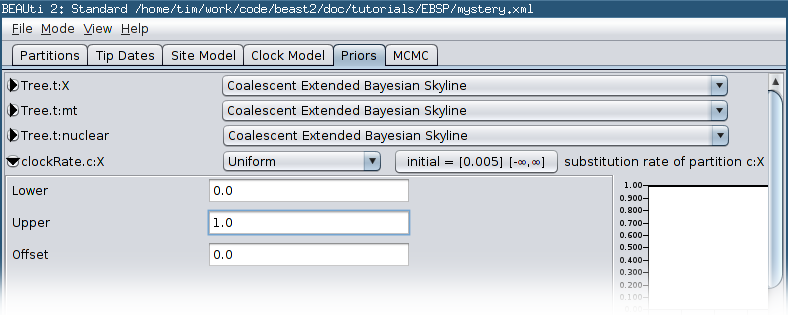
\includegraphics[width=\textwidth]{figures/clockrate_prior.png}

This should be well above any likely value for the
clock rates, but improves mixing by preventing the inference algorithm from
exploring implausible values.

Finally, we modify the hyper-prior on the mean of the population size
distribution. By default this an improper $1/x$ prior which is in general a
sensible option. Unfortunately though, this can lead to poor mixing and
necessitate runs much longer than we have time for in a tutorial such as this.
Thus, to improve the rate of convergence, we replace this with a tight Gaussian
prior centred on 1.0 with a standard deviation of 0.1. Set this by selecting
`Normal' from the drop-down menu next to populationMean.alltrees and adjusting
the parameter values as shown in the following figure:

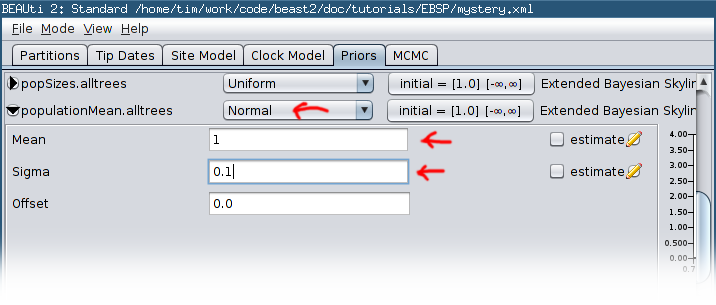
\includegraphics[width=\textwidth]{figures/popmean.png}

\subsection{Operator weights}

The MCMC algorithm used by BEAST explores the state space defined by the set of
objects (including the parameters and trees) to be inferred by applying
stochastic functions called `operators' to modify these objects. How frequently
each operator is used is defined by its `weight'. While almost any combination of (non-zero) weights will produce the same result in the end, the efficiency with which the algorithm produces effectively independent samples from the posterior can be dramatically influenced by specific choices.

To view the list of operators BEAST will use for this analysis and their
weights, select `Show operators panel' from the View menu:

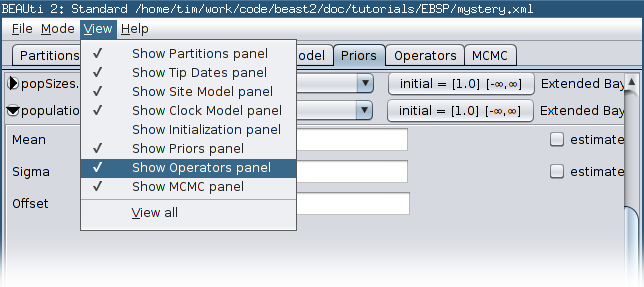
\includegraphics[width=\textwidth]{figures/view_operators.png}

The first change we make is to increase the weights of the operators affecting
the $\kappa$ parameter from theHKY substitution models from 0.1 to 3, as shown
by the three red arrows at the top of the following figure:

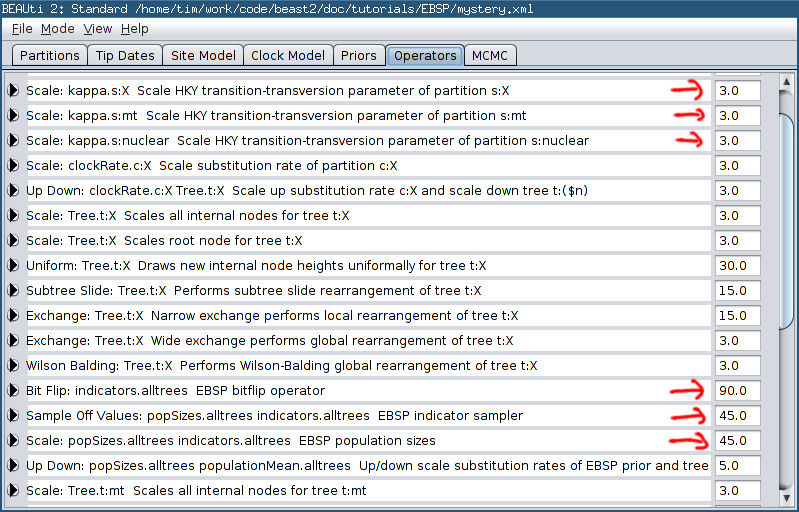
\includegraphics[width=\textwidth]{figures/operators.png}

Secondly, looking at the operators that modify each tree we see that the sum of
their weights is about 70. The sum of the default weights for the operators
affecting the population function is roughly the same at 60. Given that there
are 3 gene trees, modifications to the trees will be proposed about 3 times
more frequently than modifications to the population function.  We therefore
increase the existing population function operator weights by a factor of 3 to
even this out a bit.  To do this, modify the weights shown by the bottom three
red arrows in the previous figure.

\subsection{MCMC settings}

Finally, open the \textsc{MCMC} pane. Click the arrow to the left of `tracelog'
and change the output file name to `mystery.log', as shown in the figure below.
Similarly, click the arrow to the left of `EBSPLogger' and ensure the EBSP
output file name is `EBSP.log'.

    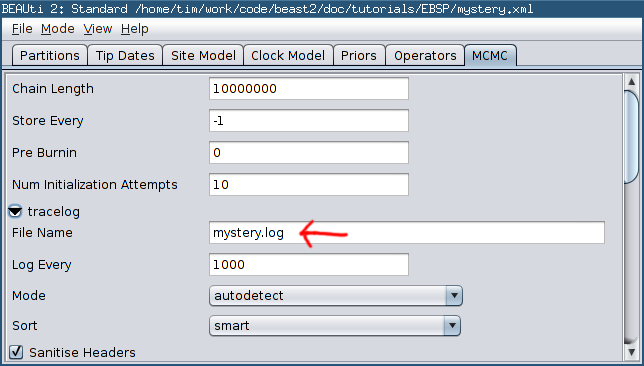
\includegraphics[width=\textwidth]{figures/mcmc_panel.png}

For this tutorial we will retain the default chain length of $10^7$ steps, but
you should note that this is almost certainly too short for a real analysis.


Once the output file names are set, create a new directory in the tutorial
folder named `mystery-run' using whatever method is appropriate under your
operating system.  Then open the BEAUti File menu and select Save, to save the
BEAST XML file representing the analysis in this new directory, using the file
name `mystery.xml'.

\section{Running, Inspecting and Plotting}

Run the chain using BEAST.\@ This takes around 5 minutes on a computer with an
Intel i5 processor, but your mileage may vary. This will generate a number of
output files that are analyzed in the following sections.

\subsection{Tracer inspection}

Start up Tracer and load the `mystery.log' file generated by the analysis.  I
suggest you browse a little on your own before reading further.

You probably looked at the posterior ESS (Effective Sample Size) first.
Selecting this and viewing its trace should reveal something similar to what is
shown below:

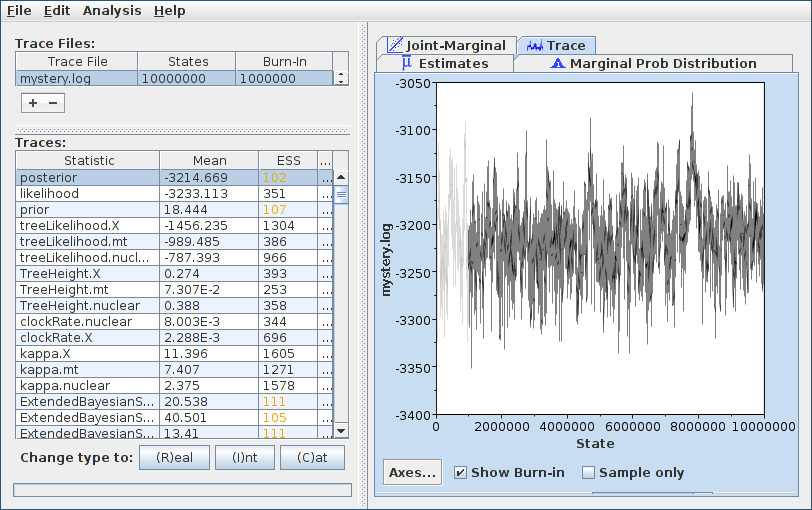
\includegraphics[width=\textwidth]{figures/tracer1.png}

The calculated value is 102, but from a visual inspection of the trace it looks
as though the true number of effectively independent samples may be even lower.
This is fine, as we knew a chain of 10 million would be too short.

The next stop for an EBSP analysis is to look at the number of population
changes. To do this, scroll to the very bottom of the table on the left-hand
side of the screen and select `sum(indicators.alltrees)'.  You should see
something similar to the following:

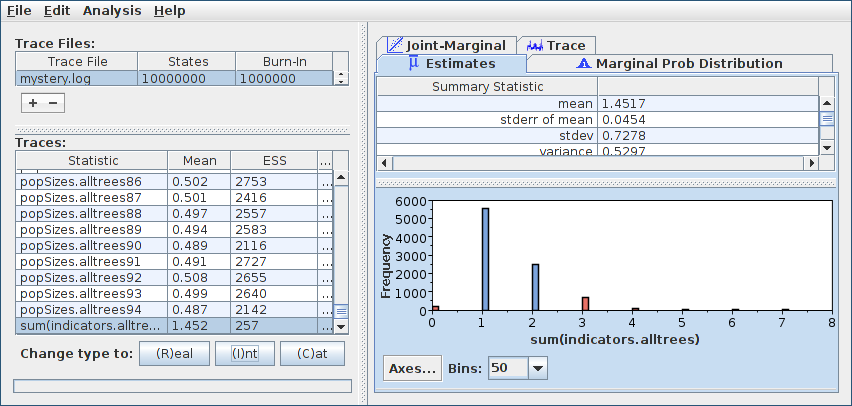
\includegraphics[width=\textwidth]{figures/tracer2.png}

This indicates that we can confidently reject a constant population since the
95\% HPD excludes 0.

Lastly, you should see that the nuclear and X clock rates come out to
approximately $8\times 10^{-3}$ and $2\times 10^{-3}$, respectively, which seem
reasonable.  The kappa values look fine, although there value for X has a very
wide credible interval indicating perhaps that there were too few substitutions
to enable a good estimate.

\subsection{Plotting}

The EBSP analysis generated a log file named `EBSP.log'.  (Remember that we set
this filename in a previous step.)  This can be used in conjunction with the
EBSPAnalyzer tool to produce a file that can be loaded into R or some other
plotting package for visualizing the demographic history posterior.

In this tutorial however, we will use an R script to produce the visualizations
directly. To do this, launch R from the `mystery-run' folder containing the
BEAST output files. (If you are using RStudio or some other graphical front-end
to R, you'll probably find a menu option to set the current working directory.)
Then execute the following from the R command line:
\begin{verbatim}
    >source("../scripts/plotEBSP.R")
    >plotEBSP("EBSP.log", useHPD=FALSE, log="y")
\end{verbatim}

The first line loads the functions defined in the R script (which is located in
the `scripts' directory in the tutorial folder). The second produces a visual
representation of the EBSP posterior samples contained in the file `EBSP.log`.
The `useHPD=FALSE' option causes plotEBSP to display 95\% Central Posterior
Density (CPD) intervals instead of HPD intervals, while the `log="y"' option
causes the y axis to be displayed using a log scale.  A figure similar to the
following will be produced:\\
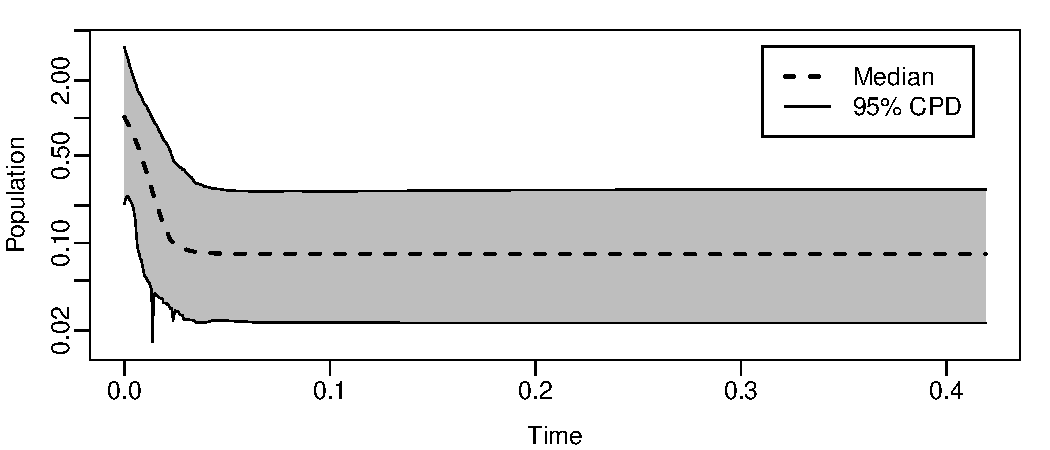
\includegraphics[width=\textwidth]{figures/mystery1.pdf}

The function accepts all of the standard R plot options allowing us to, for
instance, alter the bounds of the plot or change the axis labels or add a title
and thus is quite capable of producing publication-quality output.  For
instance, to generate a close-up with a linear vertical scale we can use
\begin{verbatim}
    >plotEBSP("EBSP.log", useHPD=FALSE, xlim=c(0, 0.03))
\end{verbatim}
which produces\\
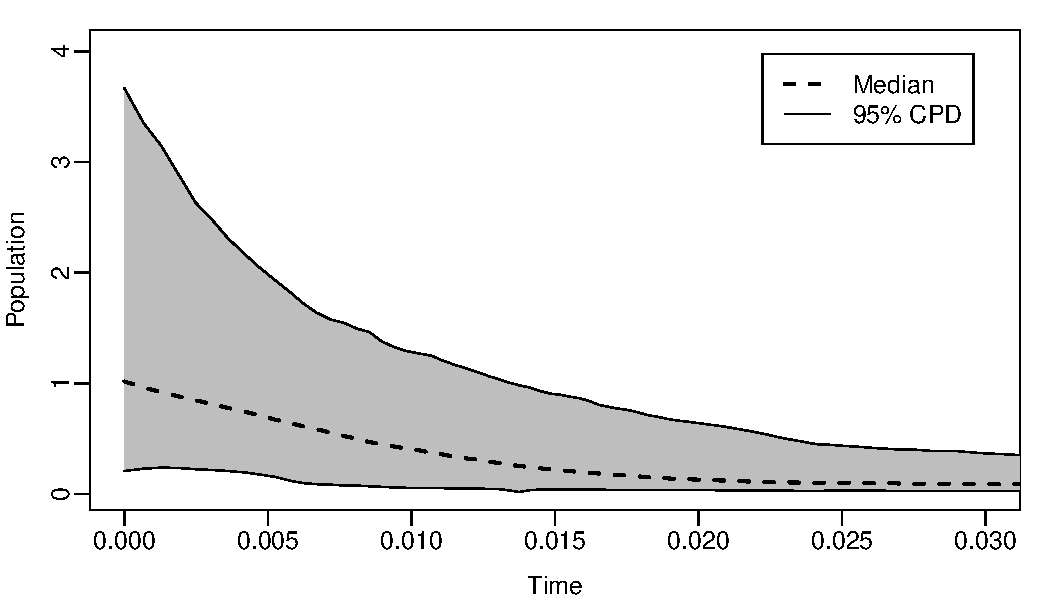
\includegraphics[width=\textwidth]{figures/mystery2.pdf}

This displays a ten-fold increase over the past 20000 years (remember our times
are in Myears). If we assume a generation time of 1 year we get a current
effective population size of around 1 million\footnote{If generation time was
    10 years, 1M years would be $10^5$ generations and so an $N_e$ of 1 would
    be $10^5$ individuals}. This is a very large number, but remember this is
for illustration purposes only. The actual numbers depend on choice of mutation
rate and generation time. Ignoring this objection, let us explore the result a
little more.

First note the wide credible intervals. Three genes will rarely give tight
bounds when dealing with population sizes. The need for more genes when
estimating effective population size can not be overemphasized. Especially when
considering that I used only 32 sequences out of a about 128. For the purpose
of this analysis the effort in sequencing this large number is wasted:
sequencing more genes, if possible, would greatly improve the results.

Secondly, recall that the EBSP prior allows the population (or rather its
slope in the case of the linear variety) to change only at points which
correspond to events on one of the gene trees.  Because these points are
generated by something akin to a coalescent process, they are not at all evenly
distributed through time.  To get an idea of their distribution, we can use
another function which is provided by the plotEBSP.R script:
\begin{verbatim}
    >plotEBSPTimesHist("EBSP.log")
\end{verbatim}
which produces the following figure:

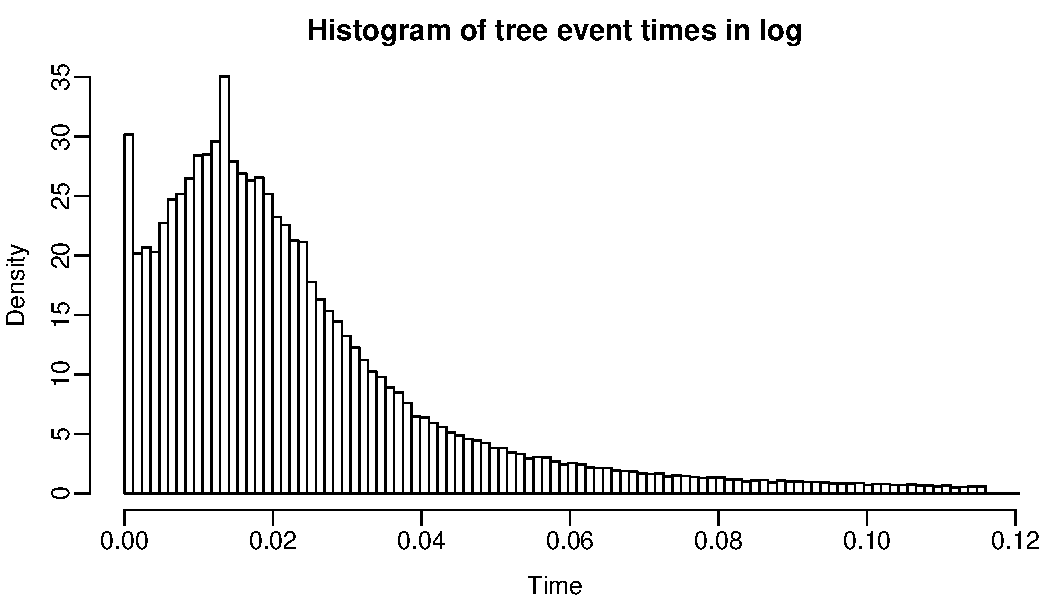
\includegraphics[width=\textwidth]{figures/mysteryTimesHist.pdf}

The spike in the histogram at time 0 is caused by the populations always having
a ``change'' point at this time.

Note the horizontal axis extends only to 0.12, in contrast with the original
skyline figure where it extended to over 0.4.  The histogram is constructed to
include 95\% of the tree event times. This figure therefore implies that there
are almost no events informing the population dynamics beyond a time of 0.1.
Thus, the apparently constant population size beyond this time is due almost
exclusively to the prior rather than the data.  One possible explanation is
that those mammals experienced a bottleneck at this point, perhaps severe
enough so that no amount of genes will let us see beyond it.

Finally, lets consider the first skyline figure. The grey area represents an
interval which includes 95\% of all population histories in the sampled
posterior.  It can be useful to look more closely at this distribution, as this
approach to summarizing the posterior can sometimes be misleading.  The
following command replaces the uniform grey shading with faint renderings of
individual population trajectories:

\begin{verbatim}
    >plotEBSP("EBSP.log", useHPD=FALSE, plotPopFunctions=TRUE, log="y")
\end{verbatim}

Note that the transparency of the population function lines can be adjusted
using the `popFunctionAlpha' parameter.

This produces the following figure, which is a full view of the posterior --
all of the samples that are summarized by the median and credible interval
lines.

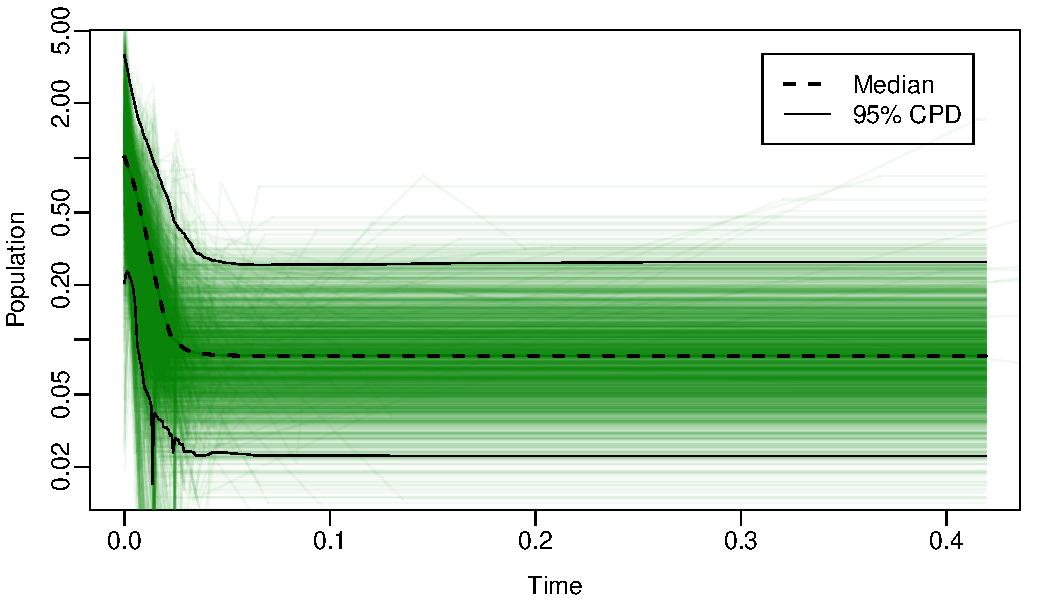
\includegraphics[width=\textwidth]{figures/mystery3.pdf}

In this case, the figure confirms that the 95\% confidence intervals are a good
representation of the actual sampled population function distribution.

\bibliography{ebsp2-tut}
\bibliographystyle{plainnat}

\end{document}
